\section{Methods}

\begin{figure}[h]
    \centering
    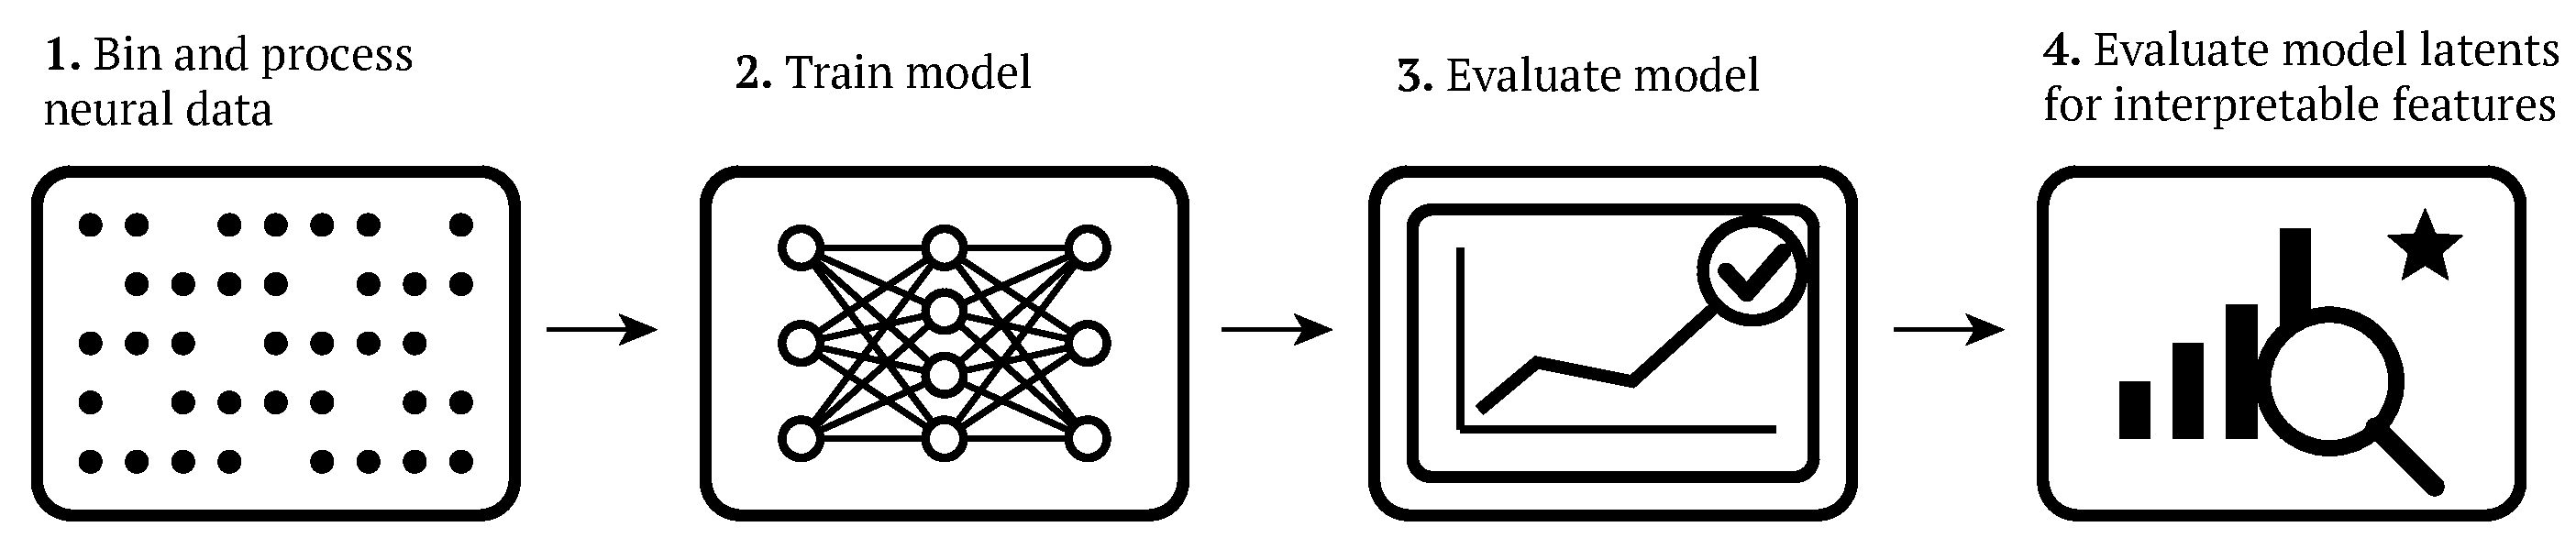
\includegraphics[width=\linewidth]{figures/mini_pipeline.pdf}
    \caption{
        \textbf{The MINI pipeline.} \\
        \small The MINI pipeline is comprised of 4 steps: 1) Spatiotemporal binning and processing of neural data; 2) Model training; 3) Model evaluation (and optional re-training); 4) Latent evaluation for feature interpretability. Steps 1-3 including model re-training, can be either semi- or fully-automated.
    }
    \label{fig:mini_pipeline}
\end{figure}

\begin{figure}[h]
    \begin{minipage}{0.64\linewidth}
    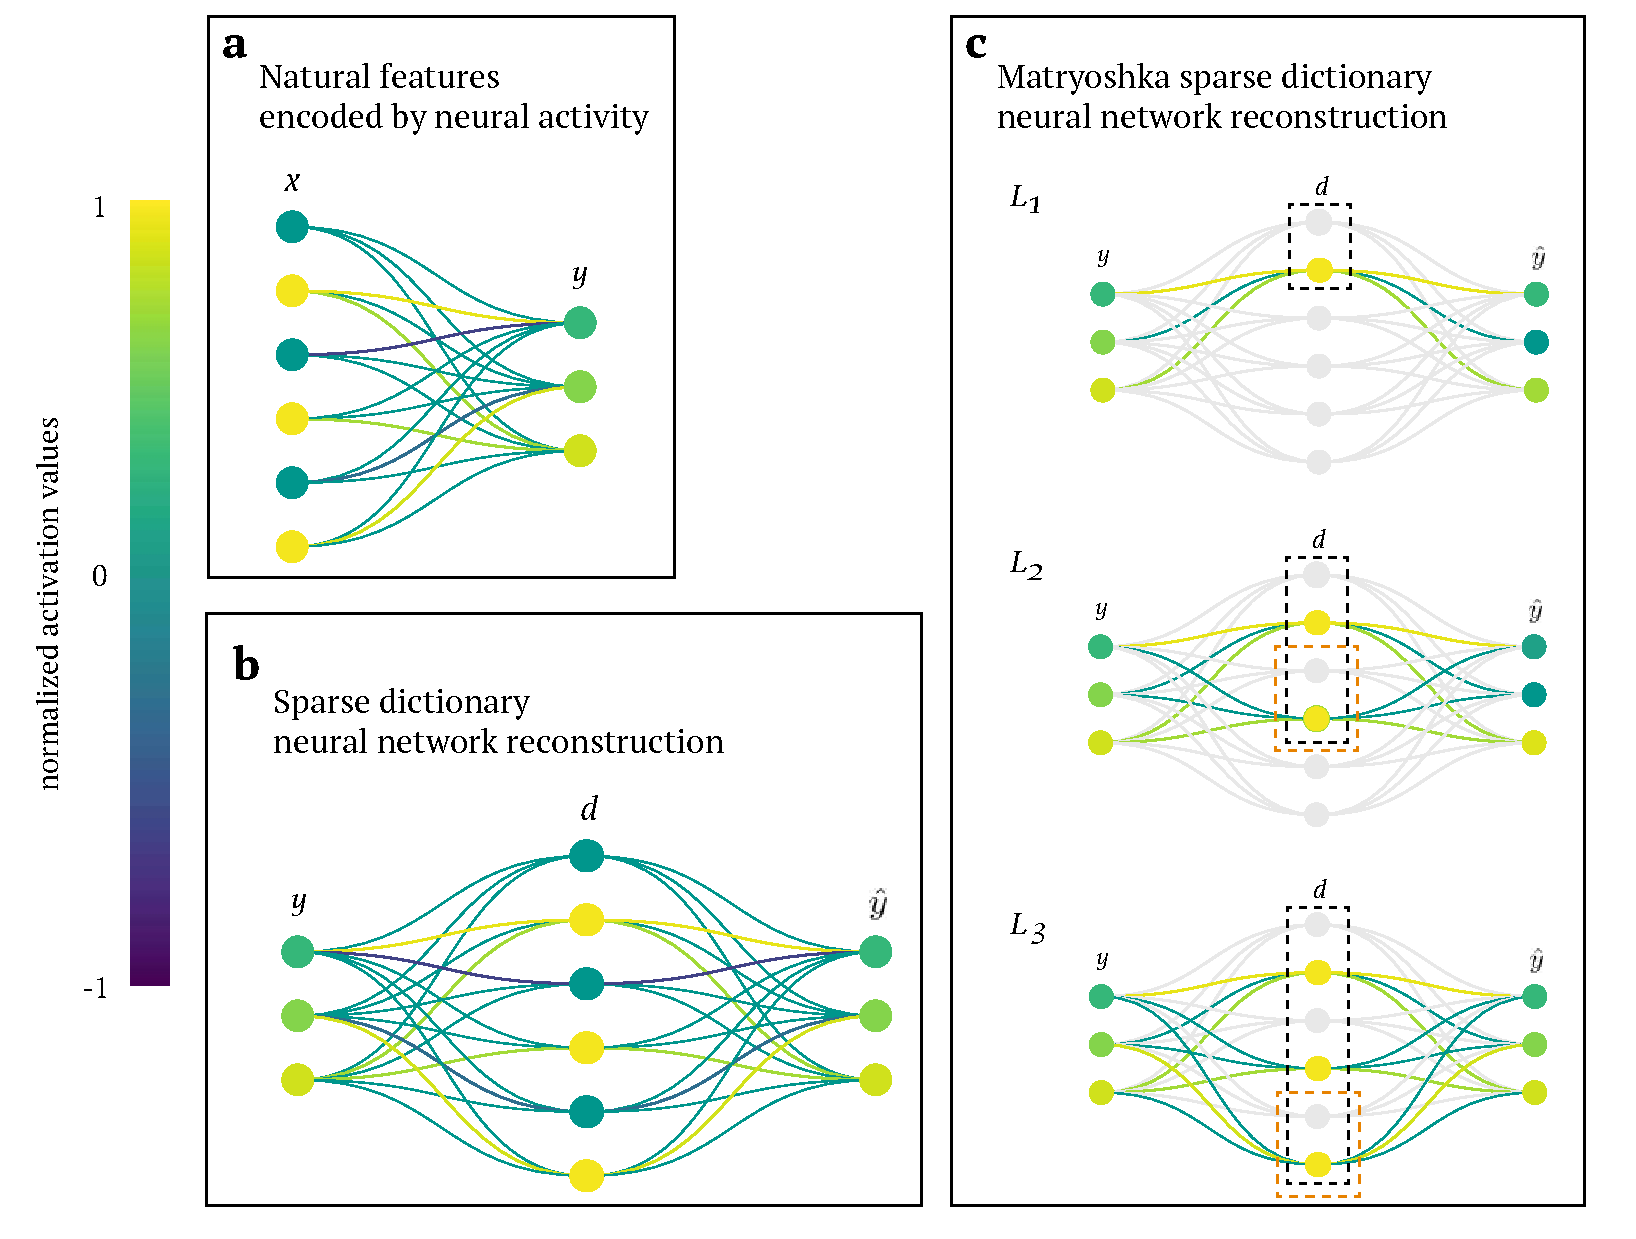
\includegraphics[width=\linewidth]{figures/sdnn_arch.pdf}
    \end{minipage}%
    \begin{minipage}{0.35\linewidth}
    \caption{
        \textbf{Model motivation} \\
        \small
        (\textbf{a}) Natural ("real-world") features $x$ get encoded by neural activity $y$. At this timepoint, three active features are simultaneously represented by the joint activity of three neurons. (\textbf{b}) A neural network reconstructs neural activity $z$ from $y$ via sparse dictionary elements $d$. When training is successful, $d$ corresponds to $x$: sparse dictionary elements represent natural features. If $z$ tries to recreate $y$ exactly ($\hat{y}$), the model is an autoencoder; in other scenarios (e.g. $z$ is separate but dependent on or related to $y$) it is a transcoder or crosscoder. (\textbf{c}) A Matryoshka spare dictionary neural network segments the latent space into multiple levels, each of which attempts to do a full reconstruction of the target neural activity. In this case, latents exclusive to the highest-level will often correspond to high-level features (e.g. a round object), while latents exclusive to the lowest-level will often correspond to low-level features (e.g. a basketball).
    }
    \label{fig:sdnn_arch}
    \end{minipage}
\end{figure}

MINI takes in high-dimensional neural data and outputs interpretable features of this data. The semi-automated pipeline consists of four steps (\autoref{fig:mini_pipeline}), the first three of which can be fully automated.

In step 1, data processing is performed to prepare the neural data for model training. MINI contains code to take the output from common spikesorters (e.g. kilosort ~\cite{pachitariu_2016_kilosort}), bin it into a 2D matrix of time X space (e.g. timebins, units (putative neurons)), and normalize the data (e.g. max normalize or z-score normalize across space (e.g. units) or time (e.g. timebins)). Users can also manually bin and process their data before proceeding to step 2.

In step 2, a SDNN is trained on the processed neural data. This step includes hyperparameter optimization, which can be done via grid search or other methods. Variant of MSAE as SAE. Transformer decoder layer. Show latex formulas for encoder, decoder, total loss.

In step 3, the trained model is evaluated using a variety of metrics to assess its performance. If the model does not meet the desired criteria, it can be re-trained with different hyperparameters. 

Finally, in step 4, the latents produced by the model are evaluated for interpretability as features. This includes visualizing their activation patterns over time and experimental conditions, as well as assessing their decoding performance. The user can then export these features for further analysis.

Example usage of the pipeline on multiple distinct datasets can be found in notebooks mentioned in \nameref{subsection:software_data_availability}.

- For a user, the full, semi-automated pipeline is as follows:
\begin{enumerate}
    \item Data processing
    \begin{itemize}
        \item Spatiotemporally bin and normalize
        \begin{itemize}
            \item MINI has a convenience function to do this directly from output of common spikesorters (kilosort), where we bin unit spikes given a specified timebin and optionally normalize (z-score or max) dataset across time and/or unit
            \begin{itemize}
                \item (and similar approach could be applied to output from common calcium imaging processing (e.g. Suite2p))
            \end{itemize}
        \end{itemize}
    \end{itemize}
    
    \item Model training
    \begin{itemize}
        \item Hyperparameter optimization
        \begin{itemize}
            \item Model parameters
            \item Optimizer parameters
        \end{itemize}
        \item By default no validation set, but can be added if we want to e.g. apply to other recordings of same animal, though this is not generally recommended (just train a freshie)
    \end{itemize}
    
    \item Model evaluation
    \begin{itemize}
        \item (We implement all metrics from SAEBench which are not language-model specific, plus a couple of our own)
        \item L0 of latents
        \item R\textsuperscript{2} (var explained) and cos sim of reconstruction-to-actual neural activity for each spatial bin, and each temporal bin
        \item Latent density histogram (as in SAEBench)
        \item Variance explained of overall reconstruction from each latent (variance shouldn't be in just a few features) ?
        \item Spectral frequency analysis to ensure temporal frequency content is preserved?
    \end{itemize}
    
    \item Feature evaluation
    \begin{itemize}
        \item When a latent is subjectively determined to be sufficiently interpretable, we call this a feature.
        \item Interactive plots showing feature activation patterns across time and experimental conditions.
        \item We evaluate its decoding performance?
        \item Export functionality.
    \end{itemize}
\end{enumerate}

For additional detail on the pipeline, see \nameref{subsection:additional_pipeline_details}.

For additional detail on model architecture, see \nameref{subsection:additional_model_details}.
